%PDFLatex
\documentclass[9pt,sansserif]{beamer}

%Latex->DVI->PS->PDF
%\documentclass[9pt,sansserif,blue,dvips,ignorenonframetext]{beamer}

%Notes: 
%\documentclass[9pt,handout,notes=show]{beamer}

%Notes only: only produces .div, so it needs previous compilation of slides mode
%\documentclass[9pt,handout,notes=only]{beamer}

%The following sets notes to use no header
\setbeamertemplate{note page}{%
  \insertnote%
}

\mode<handout>
{
\usepackage{beamerthemesplit}

\newlength{\parskipbackup}
\setlength{\parskipbackup}{\parskip}
\newlength{\parindentbackup}
\setlength{\parindentbackup}{\parindent}

\let\notebackup\note
\renewcommand{\note}[1]{\notebackup{%
	\mode<handout>{\addtocounter{page}{-1}}%
	\setlength{\parindent}{0ex}%
	\setlength{\parskip}{10pt}%
	\noindent%
	{\normalsize{}#1}%
	\setlength{\parskip}{\parskipbackup}%
	\setlength{\parindent}{\parindentbackup}%
}%
}
}

\mode<presentation>
{

%\usepackage{beamerthemesplit}
%\usepackage{beamerthemebars}
\usepackage{beamerthemelined}
%\usepackage{beamerthemetree}
%\usepackage{beamerthemetreebars}


  %1st CHOICE:
  %\usetheme{Darmstadt}
  %2nd CHOICE:
  %\usetheme{Dresden}
  %3rd CHOICE:
  %\usetheme{Warsaw}
  %\setbeamercovered{transparent}
  %4th CHOICE:
  %\usetheme{Marburg}

%\usetheme{Copenhagen}
%\usetheme{Darmstadt}
%\usetheme{Dresden}
%\usetheme{Frankfurt}
%\usetheme{Goettingen}
%
%\usetheme{Madrid} %lots of free space
%\usetheme{Malmoe} %much free space
%
%\usetheme{Marburg} %Outline right panel
%\usetheme{Montpellier}
%\usetheme{PaloAlto}	%Outline left panel
%\usetheme{Pittsburgh}
%\usetheme{Singapore}
%\usetheme{Warsaw}
}

\mode<article>
{
  %\usepackage{fullpage}
  \usepackage{pgf}
  \usepackage{hyperref}
  \setjobnamebeamerversion{beamerexample2.beamer}
}

\usepackage[english]{babel}
\usepackage[latin1]{inputenc}

\usepackage{mathptmx}
\usepackage[T1]{fontenc}

\usepackage{times}
\usepackage{amsfonts}
\usepackage{amssymb}
\usepackage{amsmath}
\usepackage{euscript}

\usepackage{color}
\usepackage{fancybox}
\usepackage{graphicx}
\usepackage{boxedminipage}
\usepackage{lscape}
\usepackage{epsfig,psfrag,graphicx}
\usepackage{url, verbatim}
\usepackage{epsfig, graphicx}
\usepackage{natbib}
\usepackage{booktabs, longtable, listings}


%% Define a new 'code' style for the url package that will use a sans serif font.
\makeatletter
\def\url@codestyle{%
  \@ifundefined{selectfont}{\def\UrlFont{\sf}}{\def\UrlFont{\sffamily}}}
\makeatother
%% Now actually use the newly defined style.
\urlstyle{code}


% ------------------------------------------------------------------------
%                      PREAMBLE 2 - Slide Background Format
% ------------------------------------------------------------------------
\newcommand{\sref}[1]{SLIDE \ref{#1}}

\definecolor{darkred}{RGB}{130,0,0}
\definecolor{darkgreen}{RGB}{0,130,0}
\definecolor{darkblue}{RGB}{0,0,130}

\newcommand{\RR}[1]{{\color{colorSG5} #1}}
\newcommand{\GG}[1]{{\color{green} #1}}
%\newcommand{\BB}[1]{{\color{blue} #1}}
\newcommand{\YY}[1]{{\color{yellow} #1}}
\newcommand{\CC}[1]{{\color{cyan} #1}}
\newcommand{\VV}[1]{{\color{violet} #1}}

%\newcommand{\BA}[1]{{\color{colorSG} #1}}
\newcommand{\BB}[1]{{\color{colorSG1} #1}}
\newcommand{\BC}[1]{{\color{colorSG2} #1}}
\newcommand{\GO}[1]{{\color{colorSG4} #1}}

\newcommand{\DR}[1]{{\color{darkred} #1}}
\newcommand{\DG}[1]{{\color{darkgreen} #1}}
\newcommand{\DB}[1]{{\color{darkblue} #1}}

\newcommand{\ce}[1]{ \vspace{-0.7cm} \begin{center} #1 \end{center} \vspace{-0.35cm} }

% CHANGED: different definition of \heading
\newcommand{\heading}[1]{\begin{center}\large\bf #1\end{center}}
\let\heading=\frametitle

% ------------------------------------------------------------------------

% ------------------------------------------------------------------------
%                               DOCUMENT
% ------------------------------------------------------------------------
% The following info should normally be given in your main file:
% [] indicates the text that is put on the bottom of each slide, remove when same as main titlepage text.

\begin{document}


\title[Agent-Based Data Analysis with Python pandas]{Agent-Based Data Analysis with Python pandas\\\bigskip FLAViz: Flexible Large-scale Agent Visualization Library}
\author[Krishna Devkota]{by Krishna Devkota\\\& Sander van der Hoog}
\date{24 Nov 2017}

\setcounter{tocdepth}{1}



%\section{Outline}   : entry in top bar
%\subsection{Outline}: entry in second bar and open dots for slides
%\frametitle{Outline}: produces a large title heading in main text field
\frame{

\begin{figure}[hbt]

\includegraphics[scale=.6]{./logos/unibi-logo-gruen.png}
\hspace{.1cm}
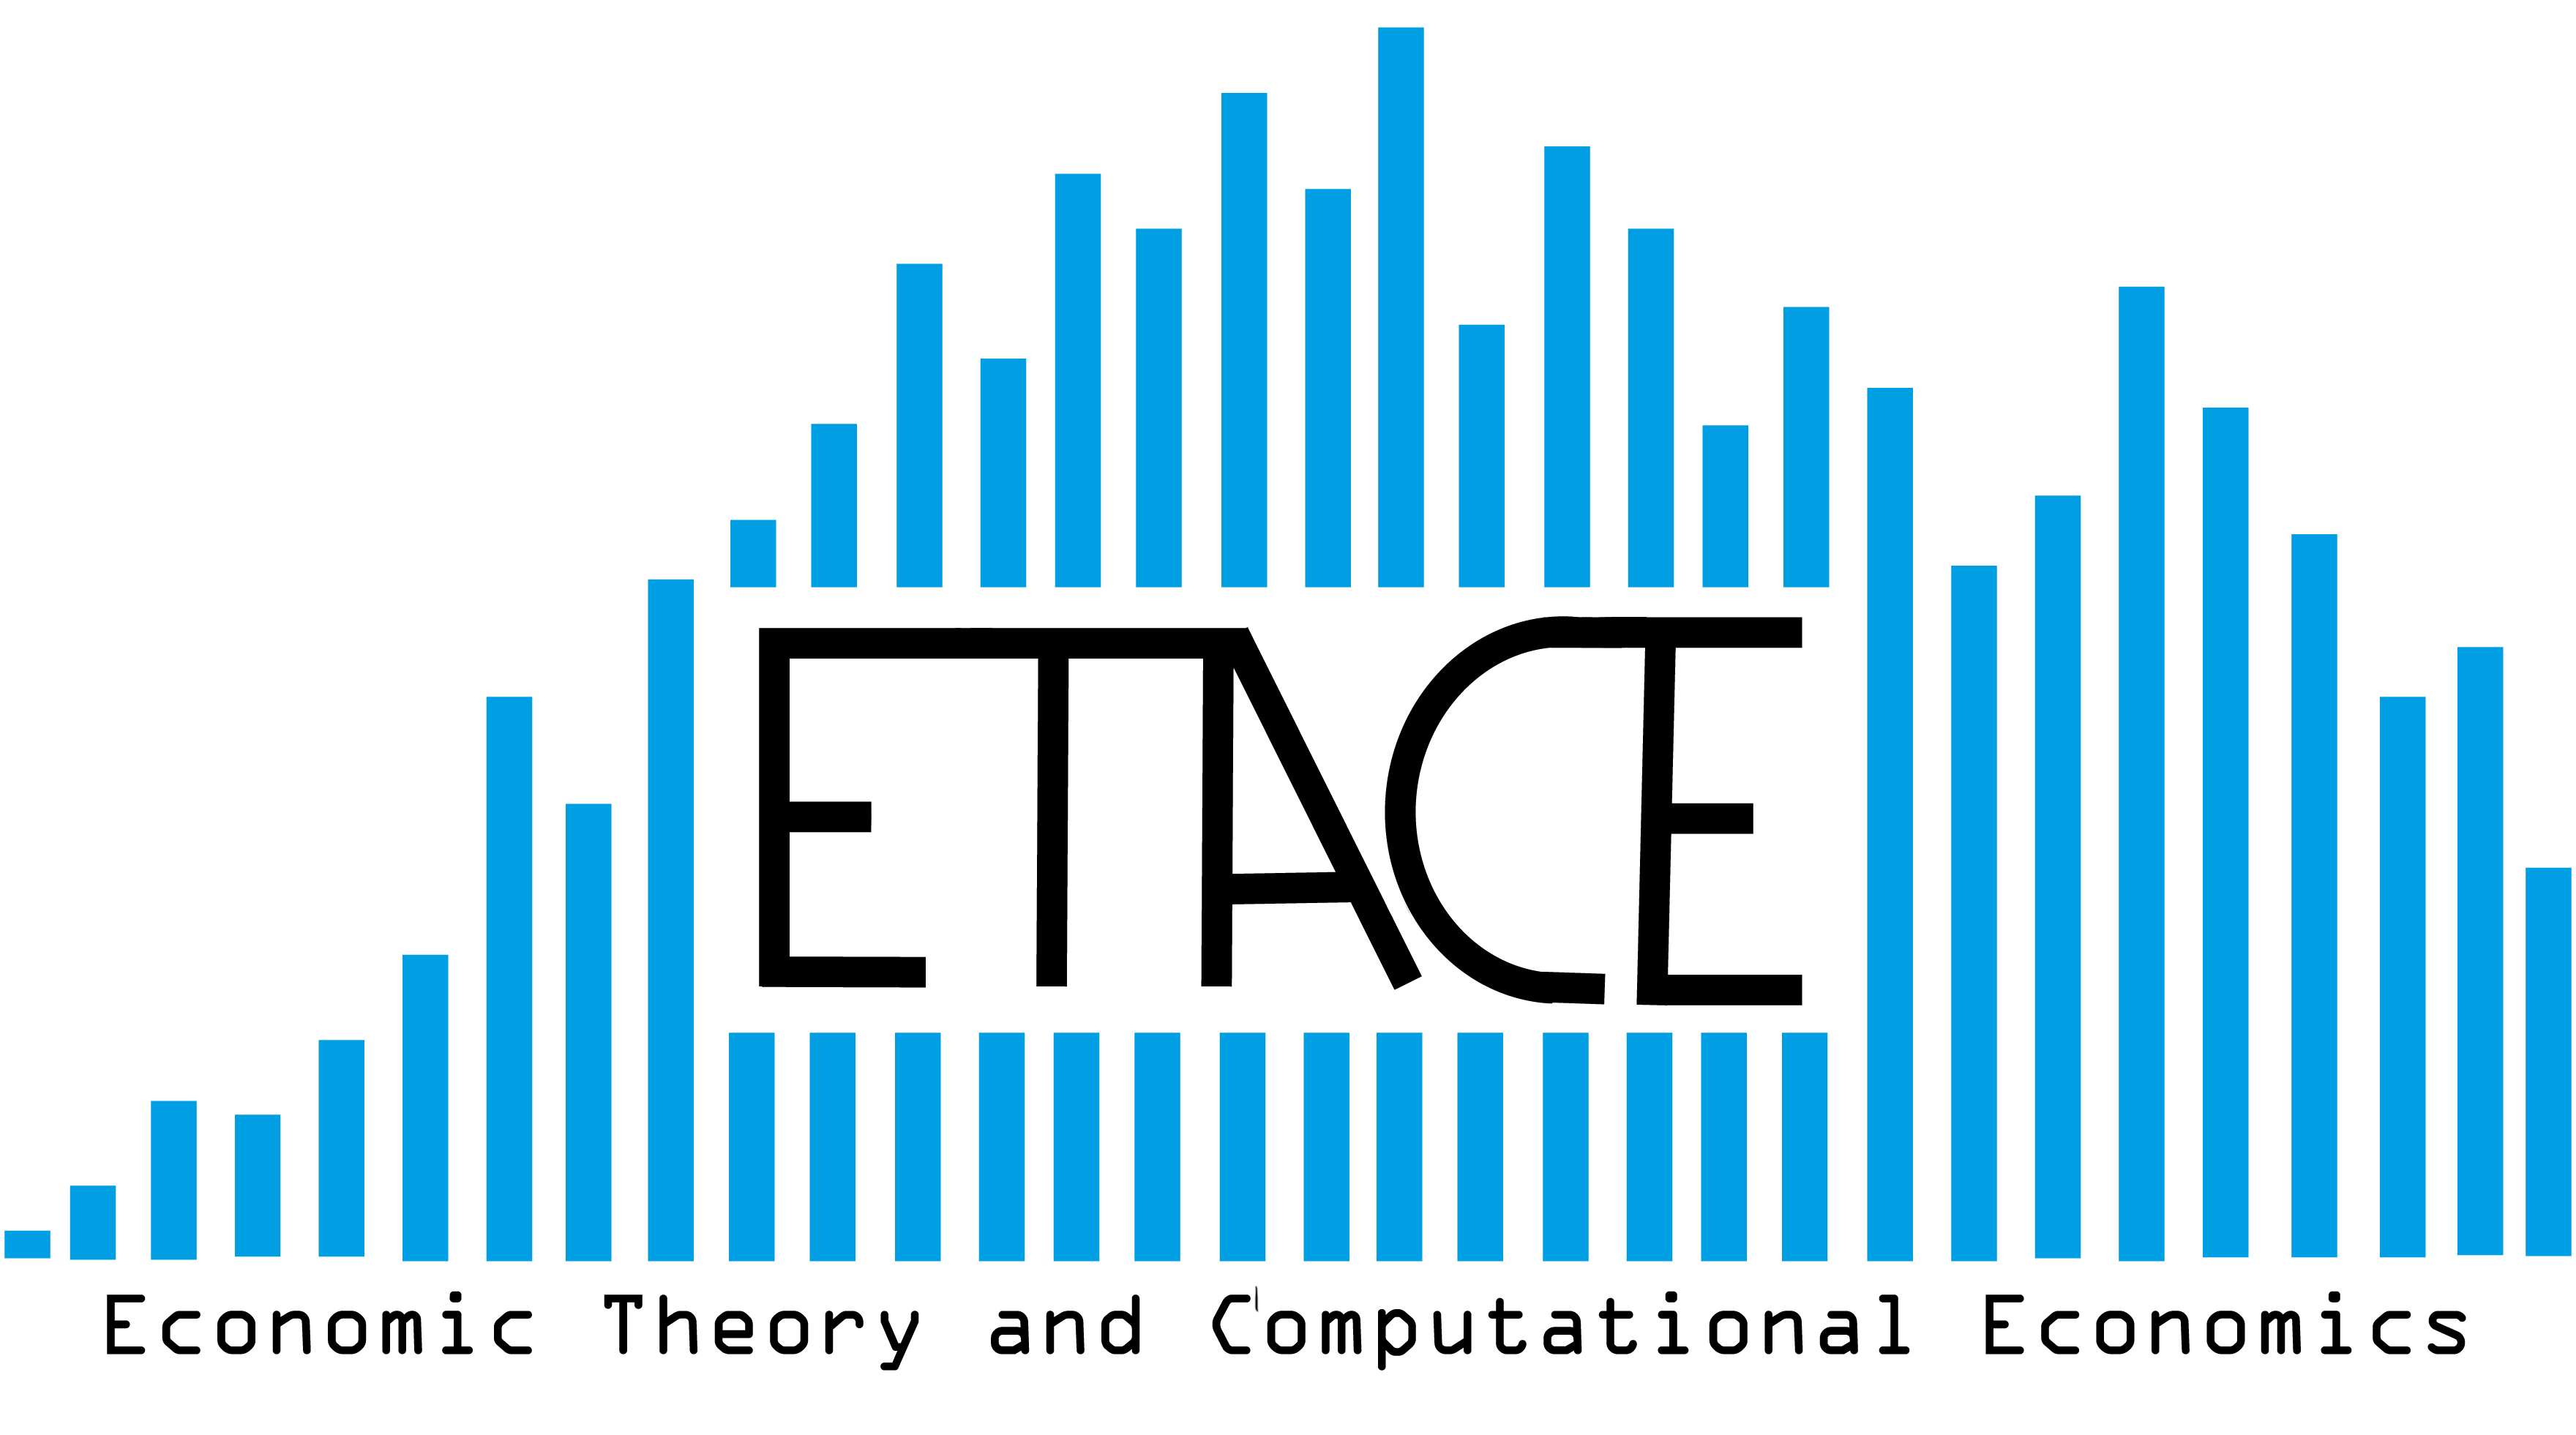
\includegraphics[scale=.02]{./logos/ETACE_new.png}
\hspace{.1cm}

\includegraphics[scale=.6]{./logos/dfg_logo_blau.jpg}
\end{figure}

\titlepage}
\note{
\small
This talk is about:
\begin{itemize}
\item A progress report on the Conquaire project, which is a DFG project on research data management and quality assurance
\item Our focus here is on economic data analysis, in particular on agent-based models and data from economic computer simulation models.
\end{itemize}
}

%--------------------------------------------------------------------------

\begin{frame}{}\small
\frametitle{Our point of departure}

\bigskip
\textbf{Continuous quality control for research data to ensure analytical reproducibility}

\bigskip
Conditions for analytical reproducibility:
\begin{itemize}
\item the primary or secondary data are available for inspection and processing
\item the data is syntactically well-formed and follows best practices from the corresponding community
\item the analytic procedures (e. g. scripts, spreadsheets, etc.) that were used to process or analyse the data are available
\item the analytic procedures can be run on the data to reproduce the actual result published in a paper.
\end{itemize}


\begin{figure}[hb!]
\centering\leavevmode
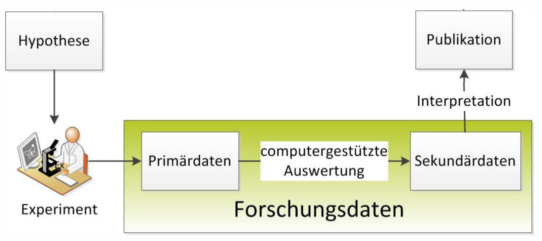
\includegraphics[scale=.75]{./png/conquaire_kick-off-meeting-slides.pdf}
\end{figure}

\end{frame}
\note{
Conquaire project:
\begin{itemize}
\item Conquaire is a DFG project at Bielefeld University on research data management and quality assurance
\item The focus is on analytical reproducibility, referring to the (computational) analysis of scientific data (can be primary or secondary data)
\end{itemize}

Conditions for analytical reproducibility:
\begin{itemize}
\item the primary or secondary data are available for inspection and processing
\item the data is syntactically well-formed and follows best practices from the corresponding community
\item the analytic procedures (e. g. scripts, spreadsheets, etc.) that were used to process or analyse the data are available
\item and: these analytic procedures can be run on the data to reproduce the actual result published in a paper.
\end{itemize}
}

%--------------------------------------------------------------------------

\begin{frame}{Agent-Based Data Analysis with pandas}\small
%\vspace{-1cm}
%\thispagestyle{empty}
%\textbf{Two ingredients central to our work flow:}

\begin{figure}[hb!]
\centering\leavevmode
\graphicspath{{../png/}}
%
\begin{minipage}{16.5cm}
%\hspace{-1cm}
%\begin{boxedminipage}{6cm}
\begin{minipage}{6cm}
\centering\leavevmode
{\bf FLAME:\\Simulation \& Data Generation}
\vspace{.5cm}\\

\includegraphics[scale=.3]{./png/flame.png}\\
\onslide<2> {\vspace{.8cm}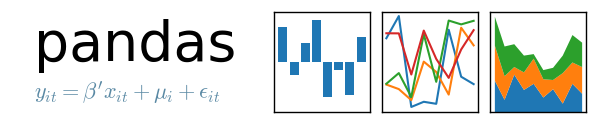
\includegraphics[scale=.25]{./png/python-pandas-screenshot.png}}
\end{minipage}
%\end{boxedminipage}
%
%\begin{boxedminipage}{5cm}
\begin{minipage}{5cm}
\centering\leavevmode
{\bf pandas:\\Data Munging \& Processing}
\vspace{.5cm}\\
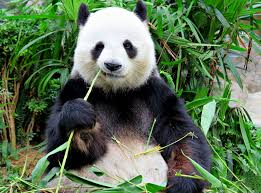
\includegraphics[scale=.5]{./png/panda-eat.jpg}\\
\end{minipage}
%\end{boxedminipage}
%
\end{minipage}
\end{figure}
\onslide<2> {\vspace{.3cm} \textbf{pandas} = Python library for scientific computing using \textbf{Pan}el \textbf{Da}ta \textbf{S}ets.\\
\textbf{Data munging} = "the process of changing data into another format so that it can be used or processed".
}
\end{frame}
\note{
Two ingredients central to our work flow:

- FLAME:\\Simulation \& Data Generation

- pandas: Data Munging \& Processing
}

%--------------------------------------------------------------------------
\section{Intro}
%--------------------------------------------------------------------------

\begin{frame}{}\small
\frametitle{What we do: Conquaire @ ETACE}

%\large
\textbf{Our primary objectives:}

\bigskip
\begin{enumerate}\itemsep2em

\item Develop a flexible and modular software library for analyzing data from ABM simulations

\item Build on pandas: a generic, general-purpose data analysis toolbox in Python

\item Toolbox components: data munging, data transformation, and data visualization

\item Create a Data Analysis Toolbox for Agent-based Simulations (DATAS)
 
\item Integrate the toolbox into an automated work-flow for research data management (primary Conquaire project mission)
 
\end{enumerate}
\end{frame}
\note{
}

%--------------------------------------------------------------------------

\begin{frame}{}\small
\frametitle{Some  plumbing of our simulation infrastructure}
%\vspace{-.6cm}
%\thispagestyle{empty}

\begin{figure}[hb!]
\centering\leavevmode
\graphicspath{{./png/}}
%
%\hspace{-4cm}
\begin{minipage}{10cm}
\centering\leavevmode
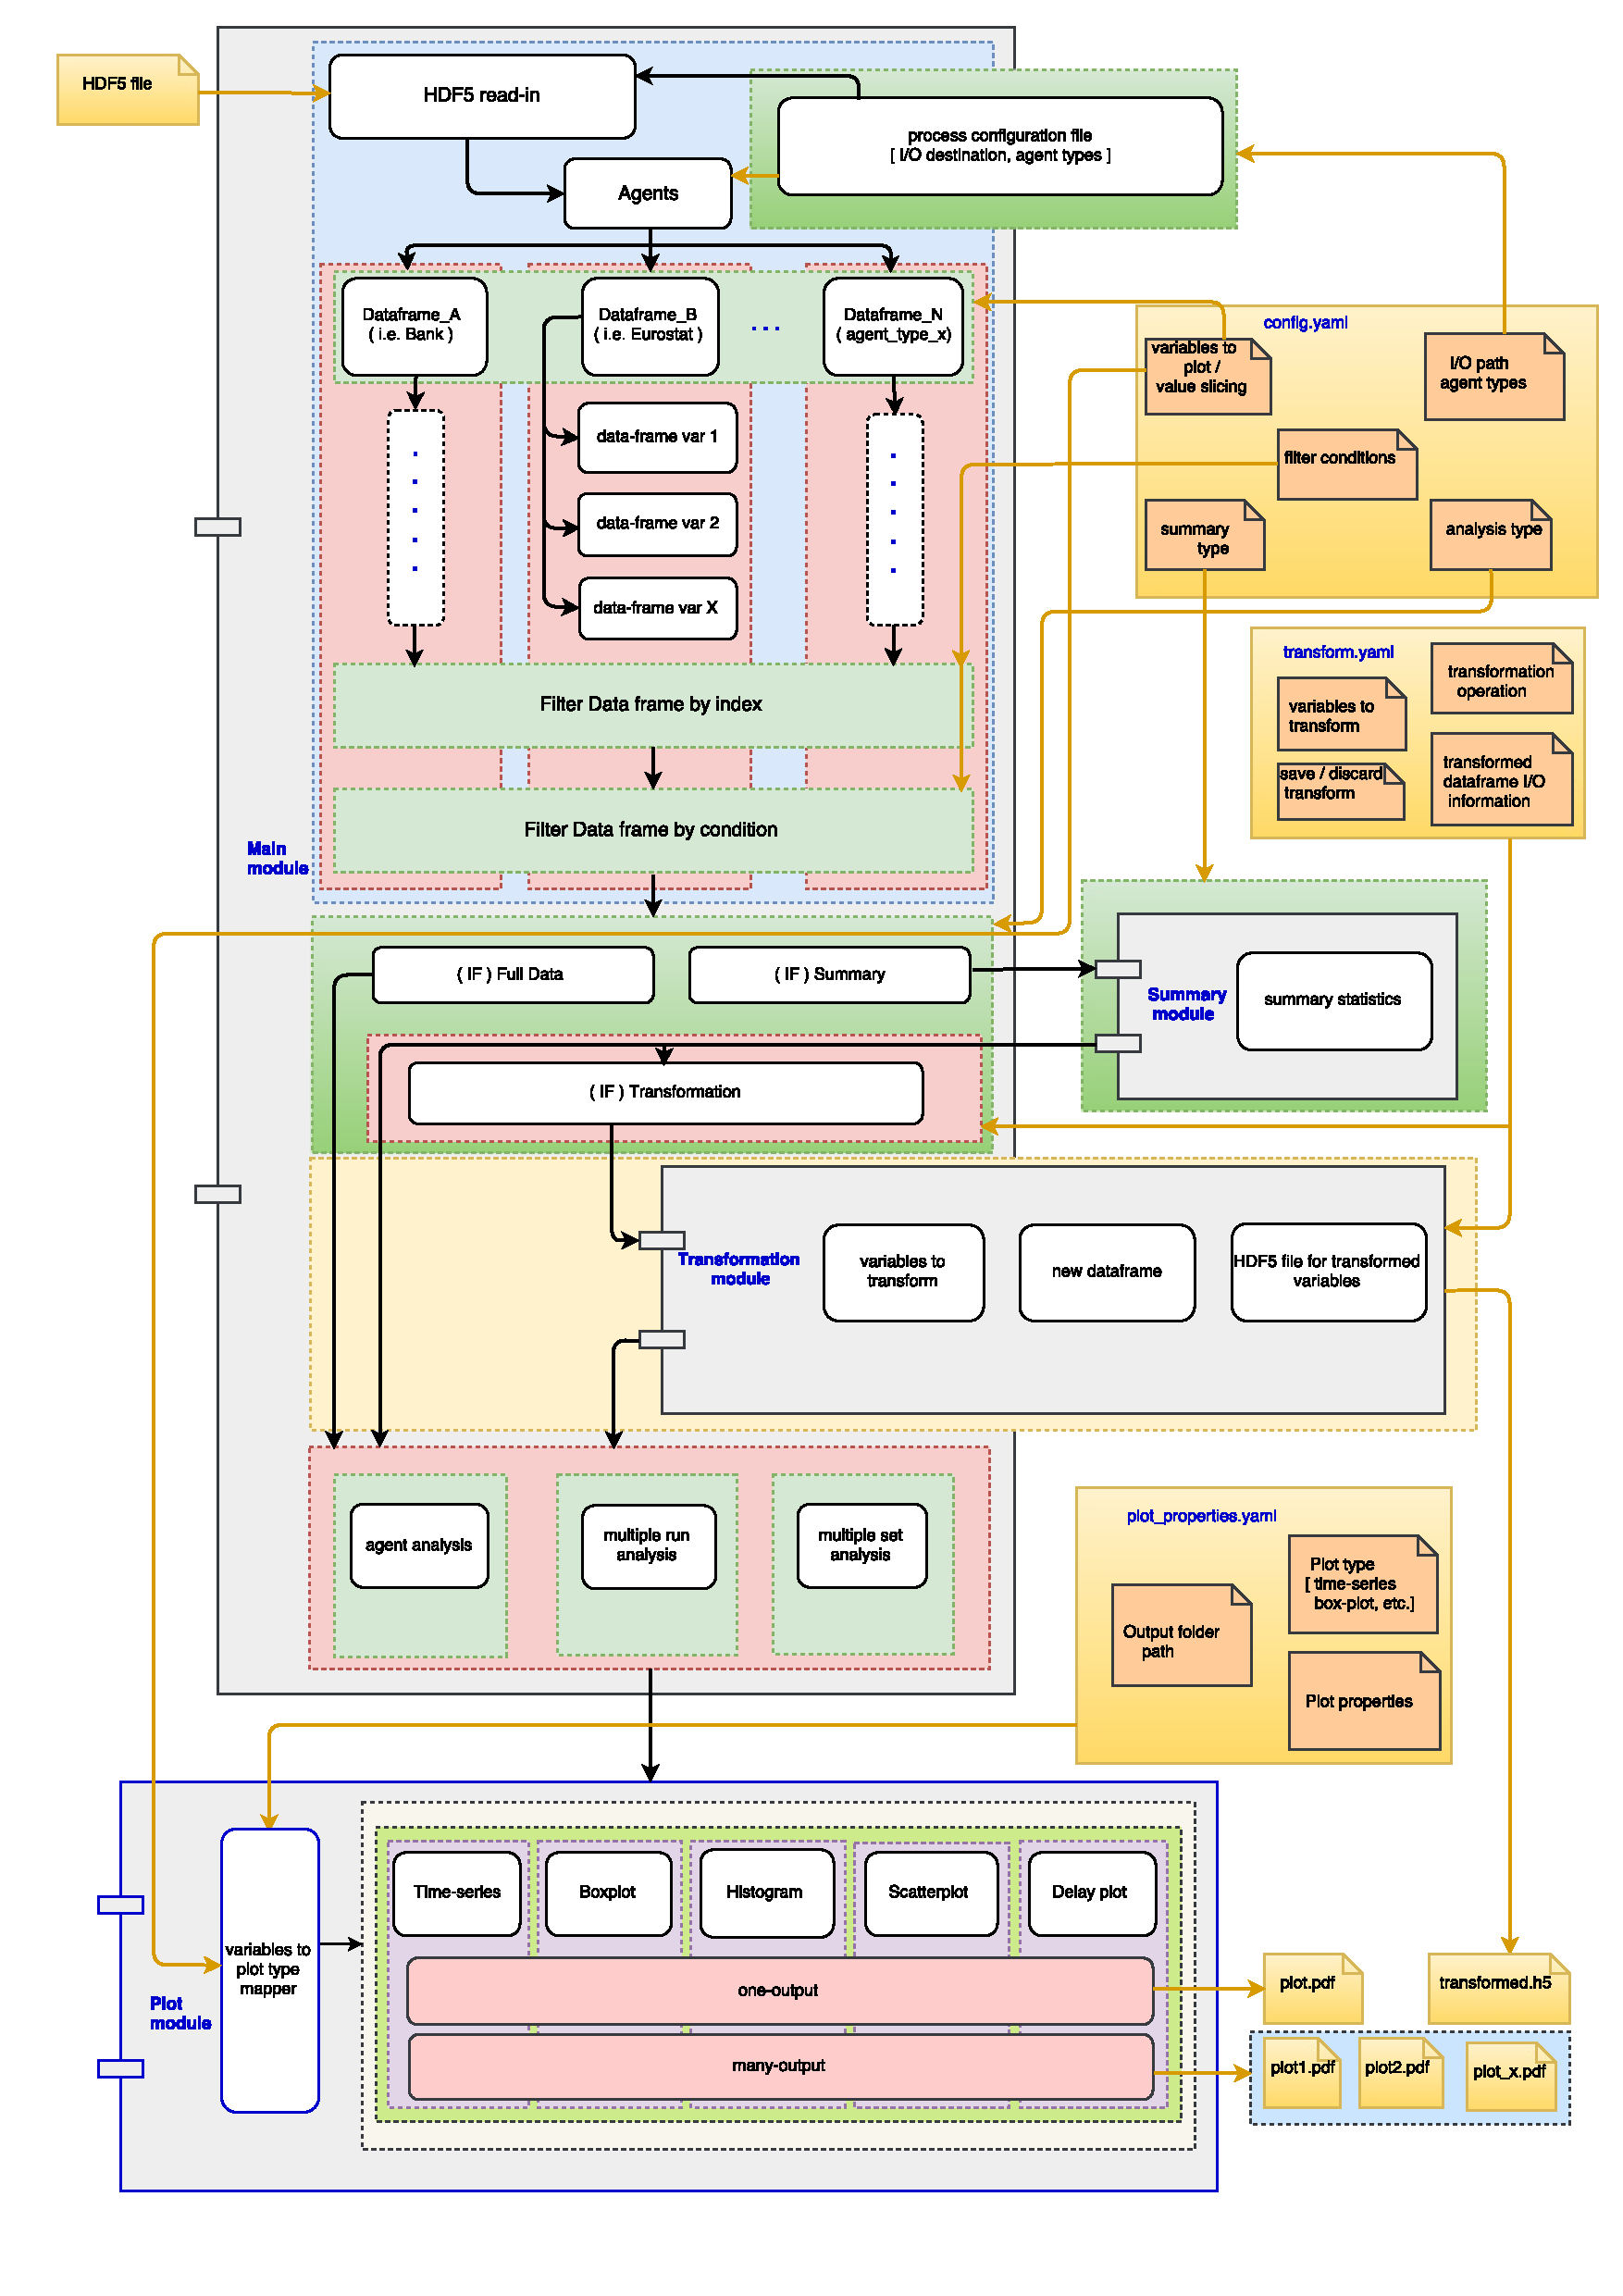
\includegraphics[scale=0.175]{flame_pandas_workflow_diagram.pdf}
\end{minipage}
\end{figure}

\end{frame}
\note{}

%--------------------------------------------------------------------------

\begin{frame}{}\small
\frametitle{Selected topics from big data analysis relevant to our purpose}

\begin{enumerate}\itemsep2em

\item Data generation

\item Data storage 

\item Data selection

\item Data filtering

\item Data transformation

\item Data visualization

\end{enumerate}
\end{frame}
\note{
Selected topics from data analytics

Each of these pose problems when confronted with large data volumes.

A concerted effort is required to tackle these issues.
}

%--------------------------------------------------------------------------
\section{Data generation}
%--------------------------------------------------------------------------

\begin{frame}{}\small
\frametitle{Data Generation, Conversion \& Storage}

\begin{figure}[hb!]
\centering\leavevmode
\graphicspath{{./png/}}
%
\hspace{-2cm}
\begin{minipage}{10cm}
%\centering\leavevmode
%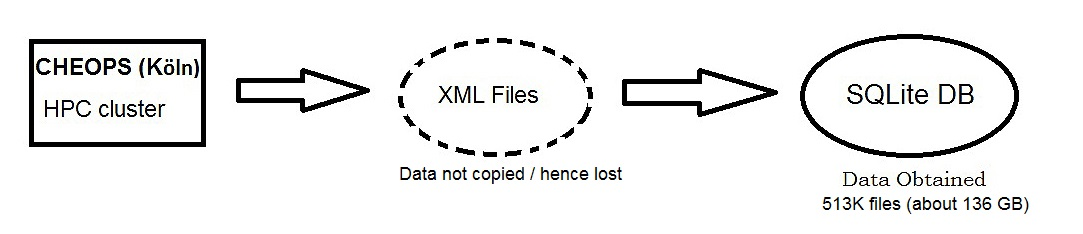
\includegraphics[scale=1]{workflow_cheops.jpg}\\ [.5cm]
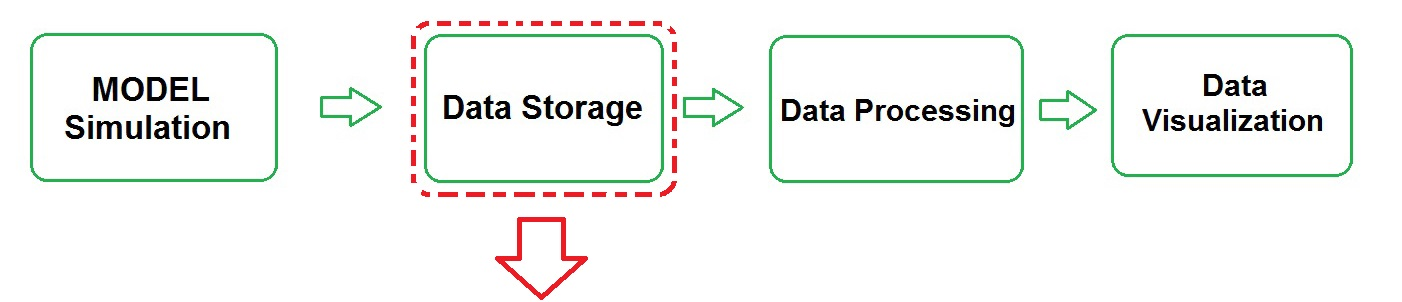
\includegraphics[scale=1]{workflow_simulation.jpg}\\
{Munging + Storage + Processing:}\\
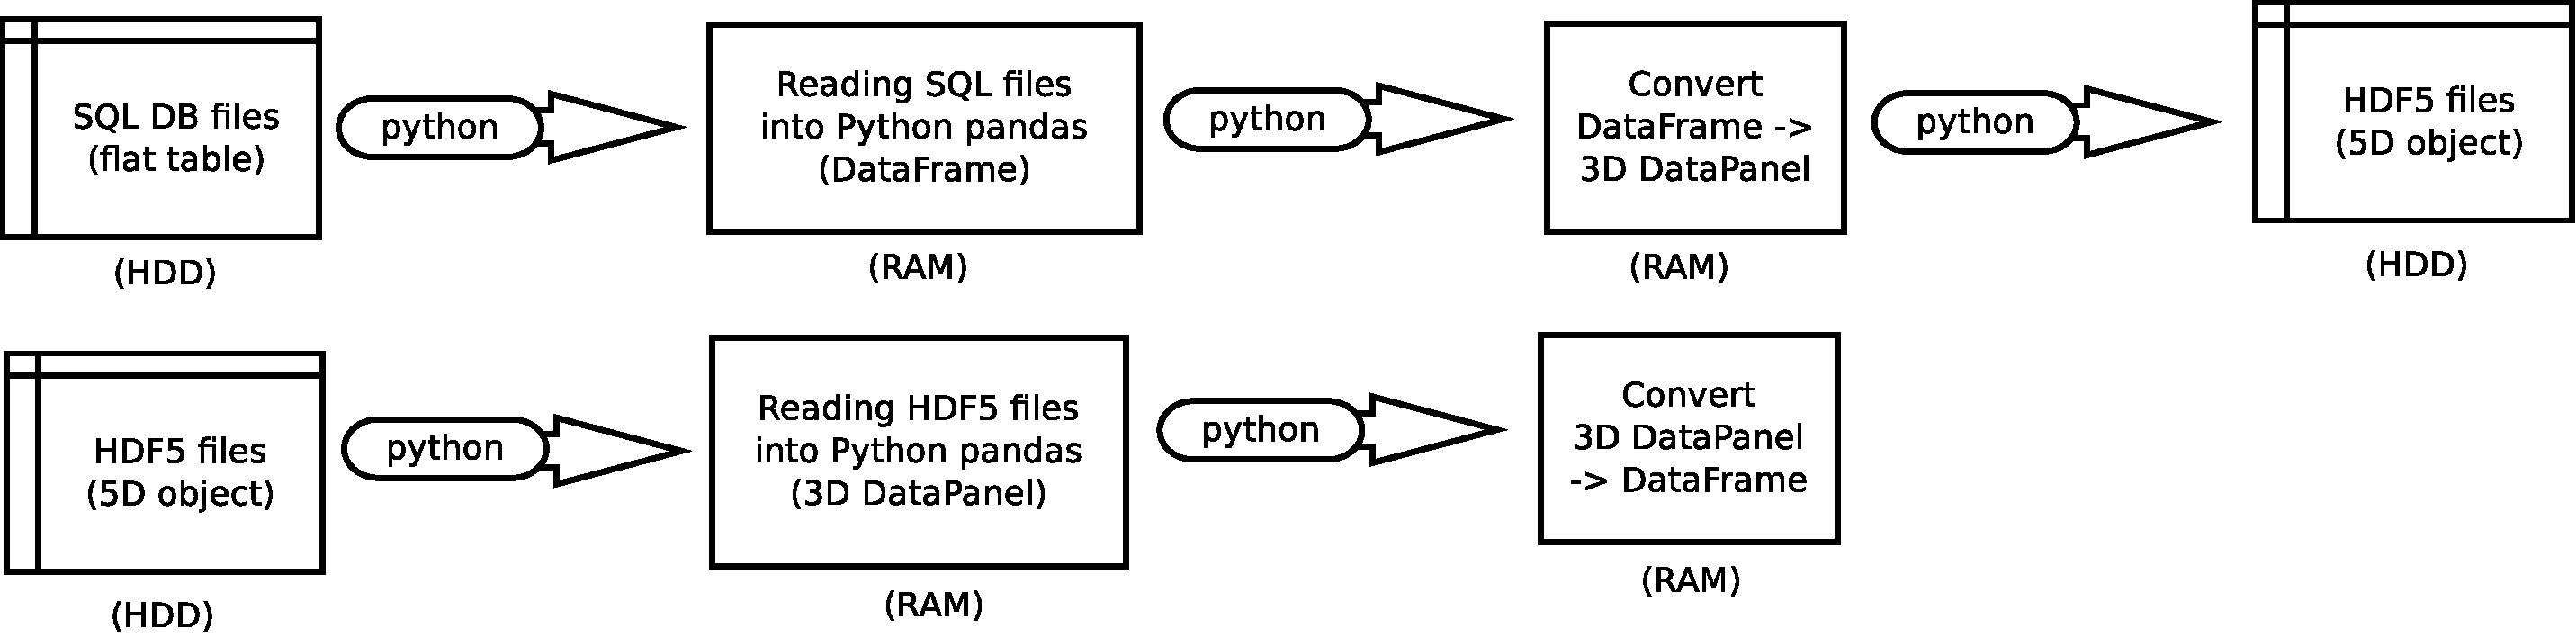
\includegraphics[scale=0.25]{workflow_data_conversion/workflow_data_conversion.pdf}
\end{minipage}
\end{figure}
\end{frame}
\note{}

%--------------------------------------------------------------------------

\begin{frame}{}\small
\frametitle{Data Volume}

\begin{minipage}{12cm}
%
\begin{minipage}{8cm}
\hspace{-2cm}
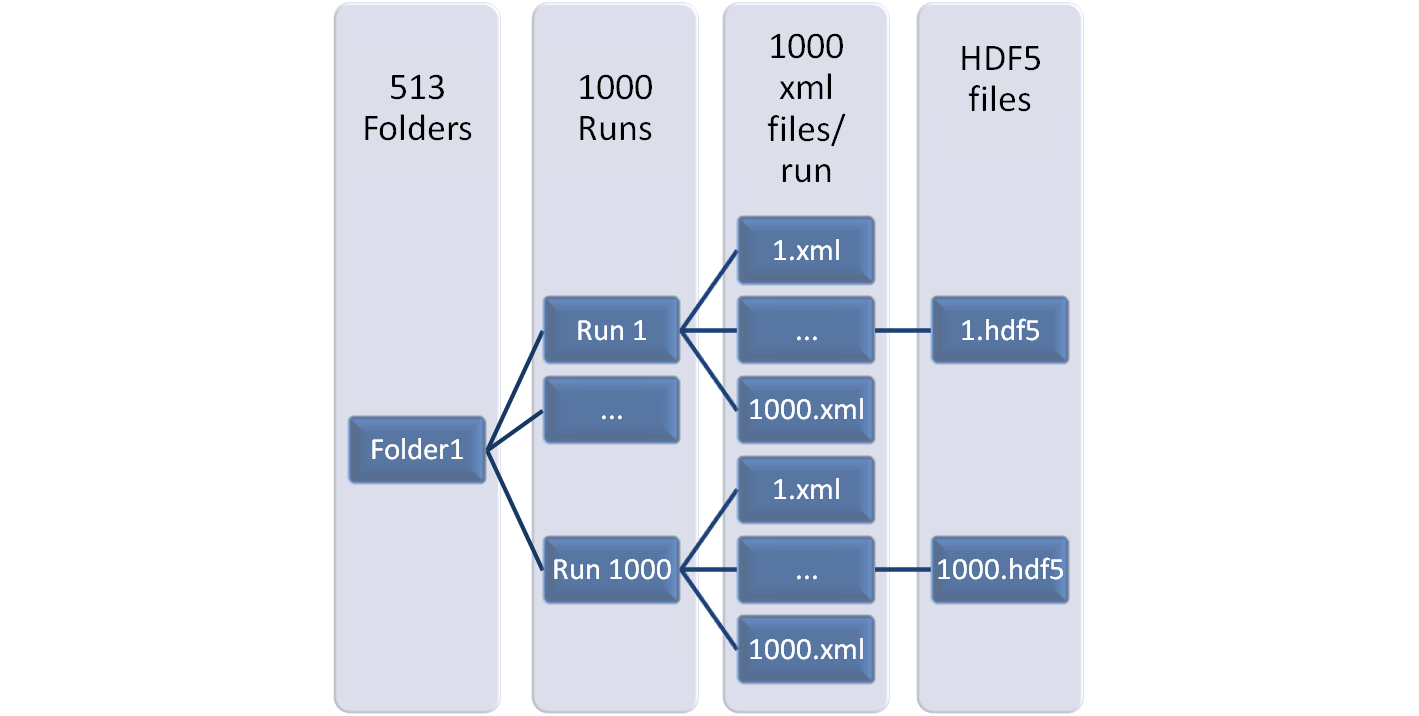
\includegraphics[scale=0.5]{./png/set_run_hierarchy.png}
\end{minipage}
%
\begin{minipage}{4cm}
{\onslide<2,3> 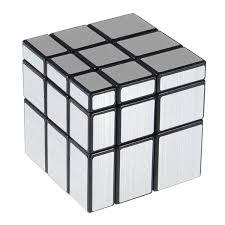
\includegraphics[scale=0.4]{./png/rubiks-mirror-cube-regular.jpg}}
%
{\onslide<3> 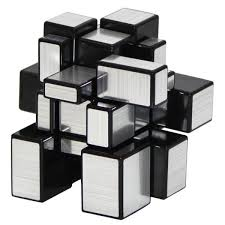
\includegraphics[scale=0.4]{./png/rubiks-mirror-cube-mixed-up.jpg}}
\end{minipage}
%
\end{minipage}

\end{frame}
\note{
\small
A particular use-case of the ABM simulations is to generate data along 3 dimensions:
\begin{itemize}
\item 513 folders for different parameter constellations
\item 1,000 runs per case
\item 1,000 XML files are generated per run
\end{itemize}

1st Rubik's Mirror Cube:

Since we have 3 dimensions of data, the data volume looks a bit like the 3D Cube as shown here.
But since the data sizes differ per run and per parameter setting, the small data blocks inside the 3D cube are not homogeneous in size.
The ideal case would be to have it all nicely ordered as structured data like the picture.

2nd Rubik's Mirror Cube:

But the real situation is more like this. The actual data is not nicely ordered, and takes up a lot of space on hard disk because it is all in separate files.
It is also not very easy to deal with when you have to read-in large volumes of data to manipulate it, or to plot something.

Typical data sizes of the various types of files are:
\begin{itemize}
\item XML files: $513x10^6$ (tiny sand grains, KB)
\item SQL files: $513x10^3$ (small beach pebbles, MB)
\item HDF5 files: 10 (big chunks of data, GB)
\end{itemize}
}

%--------------------------------------------------------------------------
\section{Data storage}
%--------------------------------------------------------------------------

\begin{frame}{}\small
\frametitle{Data storage: Our generic use-case for ABM simulations}

Agent-based data sets vary along 6 dimensions:

\bigskip
\begin{enumerate}\itemsep2em

\item Sets: $s=1,...,S$ - Parameter settings (model calibrations)

\item Runs: $r=1,...,R$ - Monte Carlo replication runs (random seeds)

\item Iterations: $t=1,..,T$ - Time periods

\item Agent types: $a=1,...,A$ - Classes, groups of agent sub-populations

\item Agent instances: $i=1,...,n_a$ - Individual agents ($n_a$= no. agents of type $a$)

\item Variables: $j=1,...,m$ - Scalars, Arrays, Composites (data structures)
\end{enumerate}

\end{frame}
\note{
}

%--------------------------------------------------------------------------

\begin{frame}{}\small
\frametitle{Data storage (cont.)}

\vspace{1cm}
A single data point (assuming a scalar variable):

{\Large
\begin{equation*}
X \in \mathbb{R}^6 \text{   or   }
X_{s,r,t,a,i,j} \in \mathbb{R}
\end{equation*}}

\bigskip
\begin{itemize}\itemsep1em
\item Requirement: keep all the data together, and in some order.

\item What type of structured data set can deal with this?\\ [5pt]

\begin{enumerate}\itemsep2em

\item \onslide<2,3,4,5> R: 2D Dataframe $\rightarrow$ not enough! $\rightarrow$ need folder hierarchy for other 4-Dims?

\item \onslide<3,4,5> pandas: 3D Panel $\rightarrow$ not enough!  $\rightarrow$ need folder hierarchy for other 3-Dims?

\item \onslide<4,5> HDF5: Hierarchical data format v5  $\rightarrow$ could this be enough? 
\begin{itemize}
\item \onslide<5> Data group / data subgroup / data set (POSIX standard)
\end{itemize}

\end{enumerate}
\end{itemize}

\end{frame}
\note{
}

%--------------------------------------------------------------------------

\begin{frame}{}\small
\frametitle{Data storage: Revised data hierarchy}

\begin{enumerate}\itemsep1em

\item {\color{darkgreen}Agent types: $a=1,...,A$} - Classes, groups of agent sub-populations

\item \hspace{1cm}{\color{darkblue}Sets: $s=1,...,S$} - Parameter settings (model calibrations)

\item \hspace{1cm}{\color{darkblue}Runs: $r=1,...,R$} - Monte Carlo replication runs (random seeds)

\item \hspace{2cm}{\color{darkred}Iterations: $t=1,..,T$} - Time periods

\item \hspace{2cm}{\color{darkred}Agents: $i=1,...,n_a$} - Individual agents (per type)

\item \hspace{2cm}{\color{darkred}Variables: $j=1,...,m$} - Scalars, Arrays, Composites
\end{enumerate}

\bigskip
{\color{darkgreen}HDF5 file}: 1 file per agent type: Eurostat, Firm, Household, Bank, ...

\bigskip
{\color{darkblue}Data groups inside a HDF5 file}: 
\begin{itemize}
\item flat form:  \url{set_1_run_1}, \url{set_1_run_2}, ...
\item data hierarchy: \url{set_1/run_1}, \url{set_1/run_2}, ...
\end{itemize}

\bigskip
{\color{darkred}pandas 3D Panel}: homogeneous data block inside each data group

\end{frame}
\note{
}

%--------------------------------------------------------------------------
\section{Data processing}
%--------------------------------------------------------------------------

\begin{frame}{}\small
\frametitle{Data processing: HDF5 (HDD) $\rightarrow$ DataFrame in pandas (RAM)}

\bigskip
\begin{enumerate}\itemsep2em

\item Python pandas: 
	\begin{itemize}\itemsep1em
	\item read-in HDF5 file per agent type into a DataFrame in RAM (parallelizable!)
	\item create a flattened DataFrame with hierarchical-index for each agent type
	\item 6D data: 5-dim hierarchical index for other 5 dimensions
	\item select type of analysis (agent-level, run-level, set-level)
	\item use groupby, filter, transform to manipulate data in RAM
	\item create summary statistics
	\end{itemize}

\item Store data transformations in temporary DataFrame in RAM

\item Create visualizations: time series, box plots, histograms, scatter plots

\item Write out final data to disk: hdf5, png, pdf, csv
 
\end{enumerate}
\end{frame}
\note{
}

%--------------------------------------------------------------------------

\begin{frame}{}\small
%\frametitle{}
\vspace{-1cm}
\thispagestyle{empty}

\begin{figure}[hb!]
\centering\leavevmode
\graphicspath{{./png/}}
%
\hspace{-4cm}
\begin{minipage}{10cm}
\centering\leavevmode
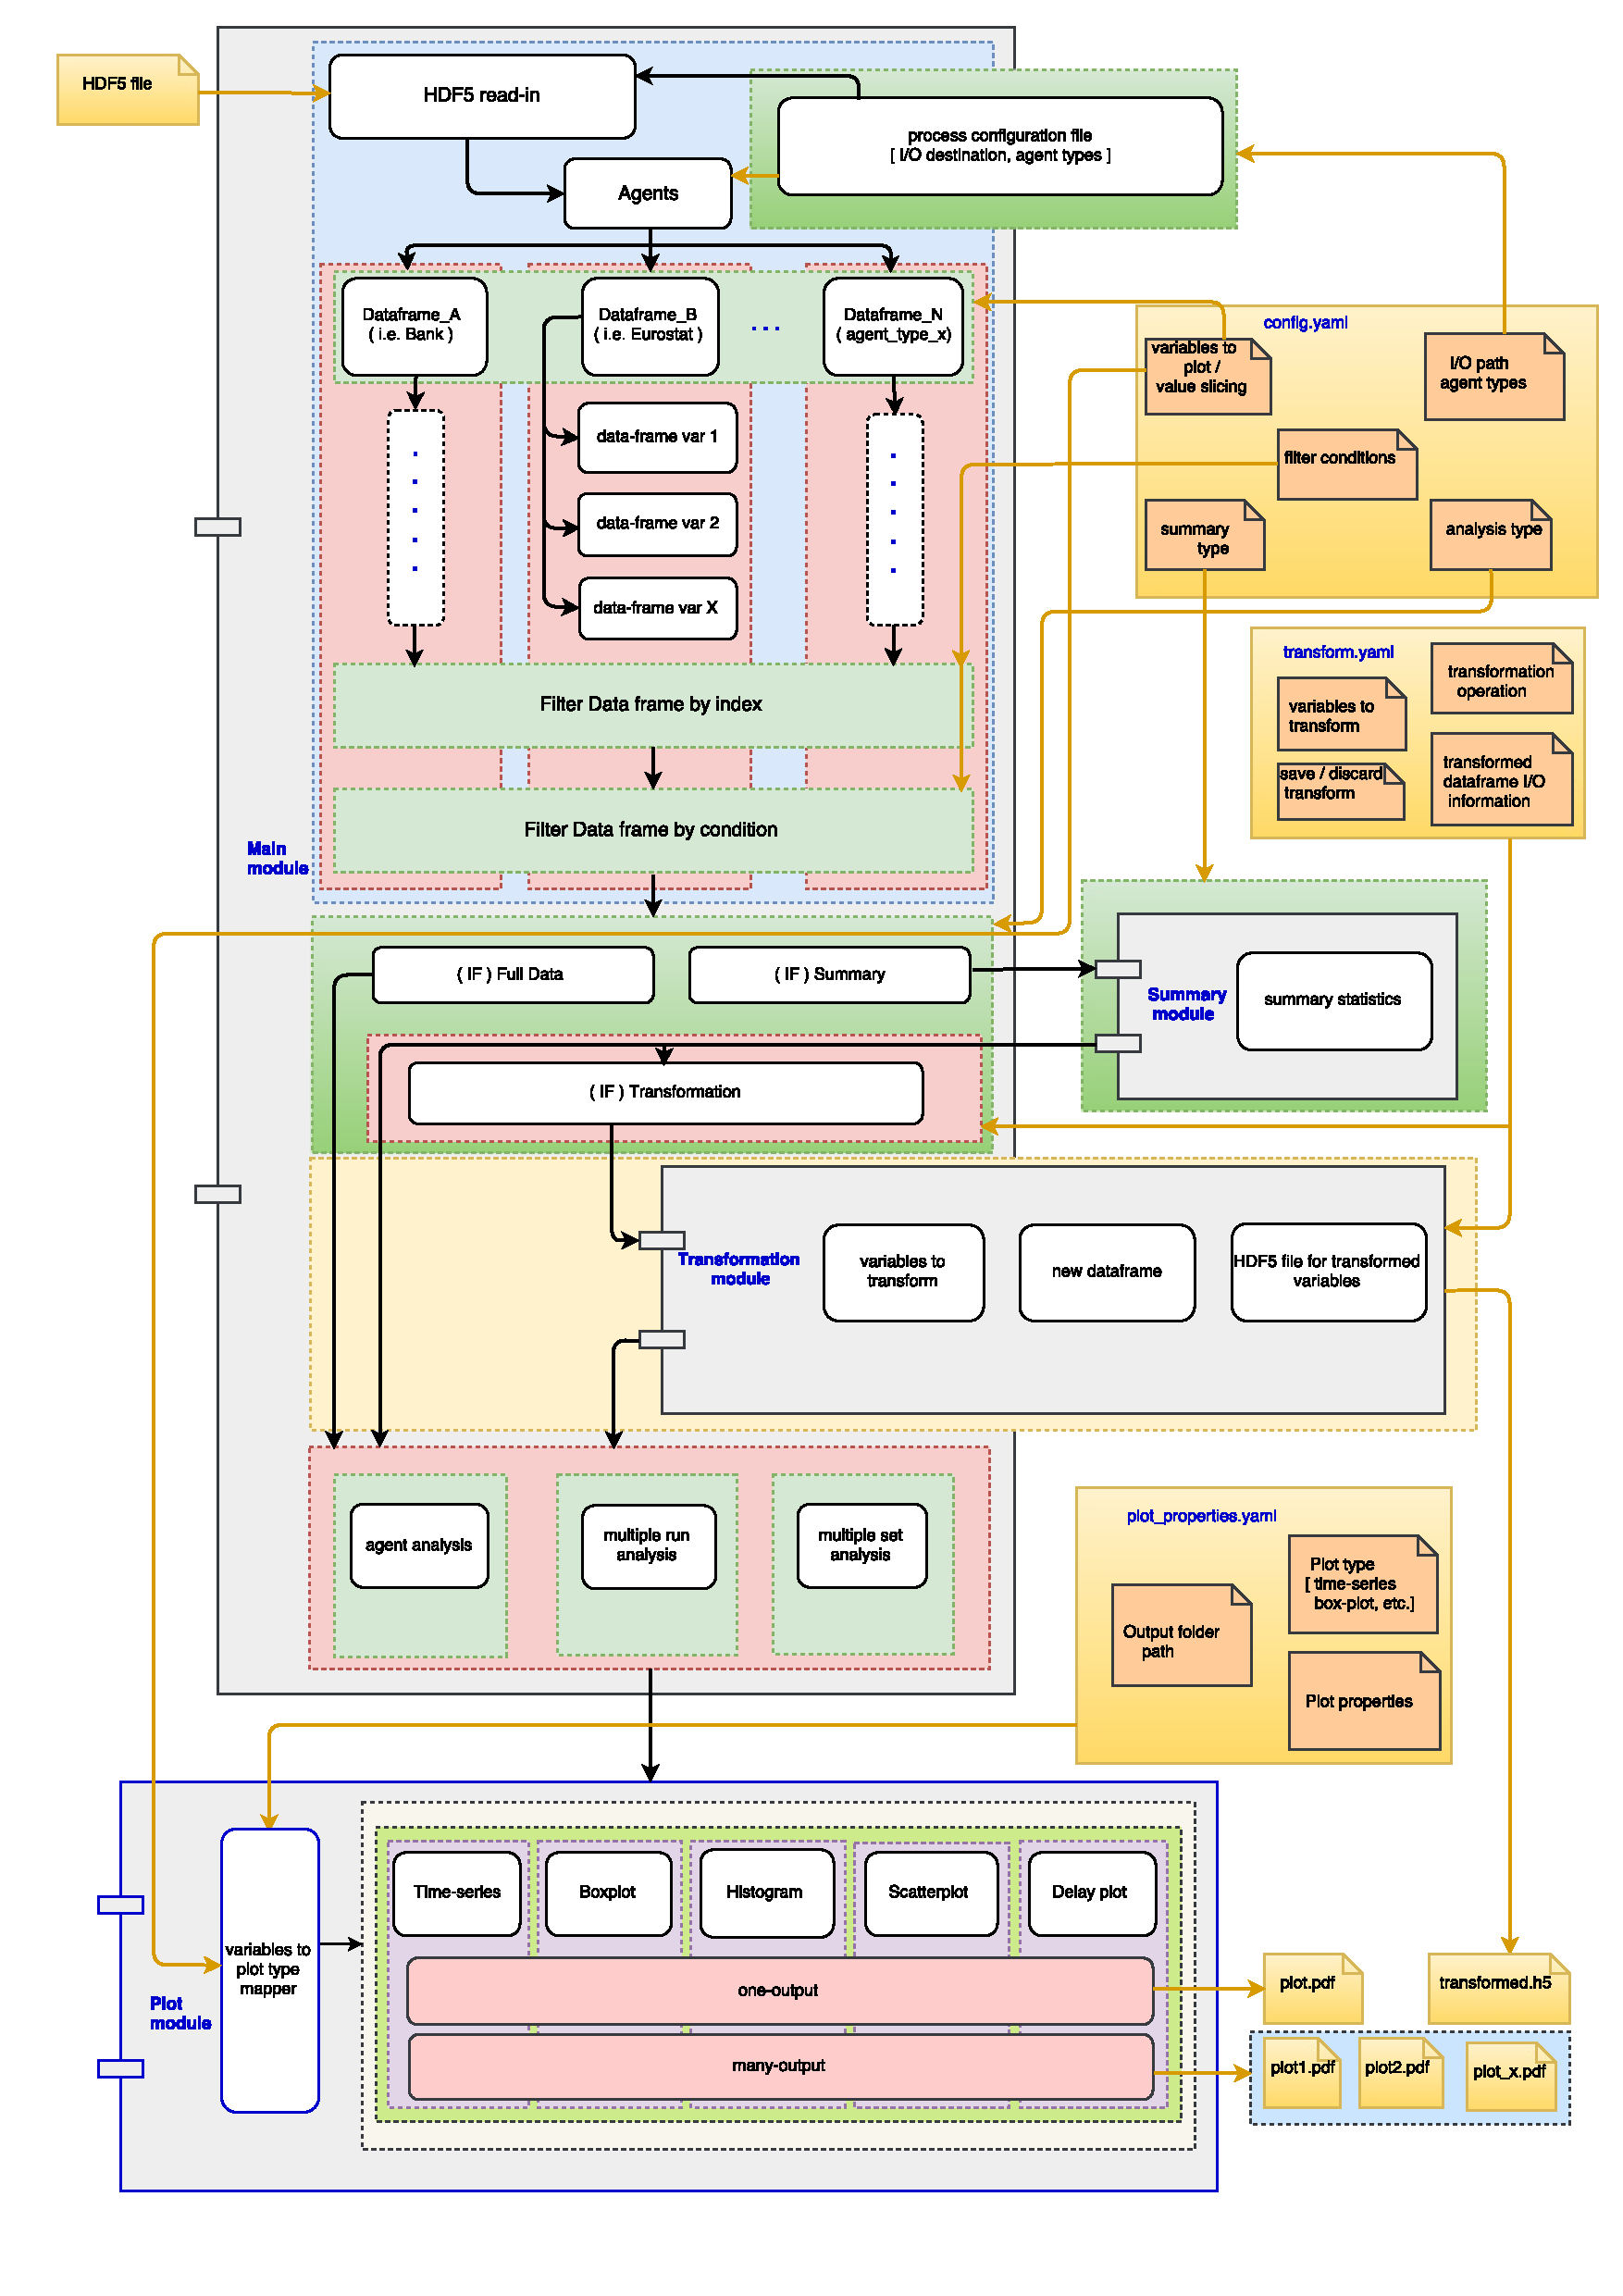
\includegraphics[scale=0.45]{flame_pandas_workflow_diagram.pdf}
\end{minipage}
\end{figure}

\end{frame}
\note{
\textbf{Flame with pandas workflow diagram}

\underline{Module Blue:} Data input module

a. Read-in from HDF5, loop across agent types

\underline{Module Green:} Data preparation module

b. In RAM, create a data frame for each agent type to hold all agent instances of that type

\underline{Module Red:} Data selection module

c. Data selection: filter the data according to a list of variables for each agent type

d. Data filtering: filter the data according to filter criteria (X>0, ID==2,...)

\underline{Module Green:} Data aggregation module

e. Data aggregation: create summary statistics of the data

f. Pass filtered data frame with summary statistics (in RAM) to the next modules
}

%--------------------------------------------------------------------------

\begin{frame}{}\small
%\frametitle{}
\vspace{-7.7cm}
\thispagestyle{empty}

\begin{figure}[hb!]
\centering\leavevmode
\graphicspath{{./png/}}
%
\hspace{-4cm}
\begin{minipage}{10cm}
\centering\leavevmode
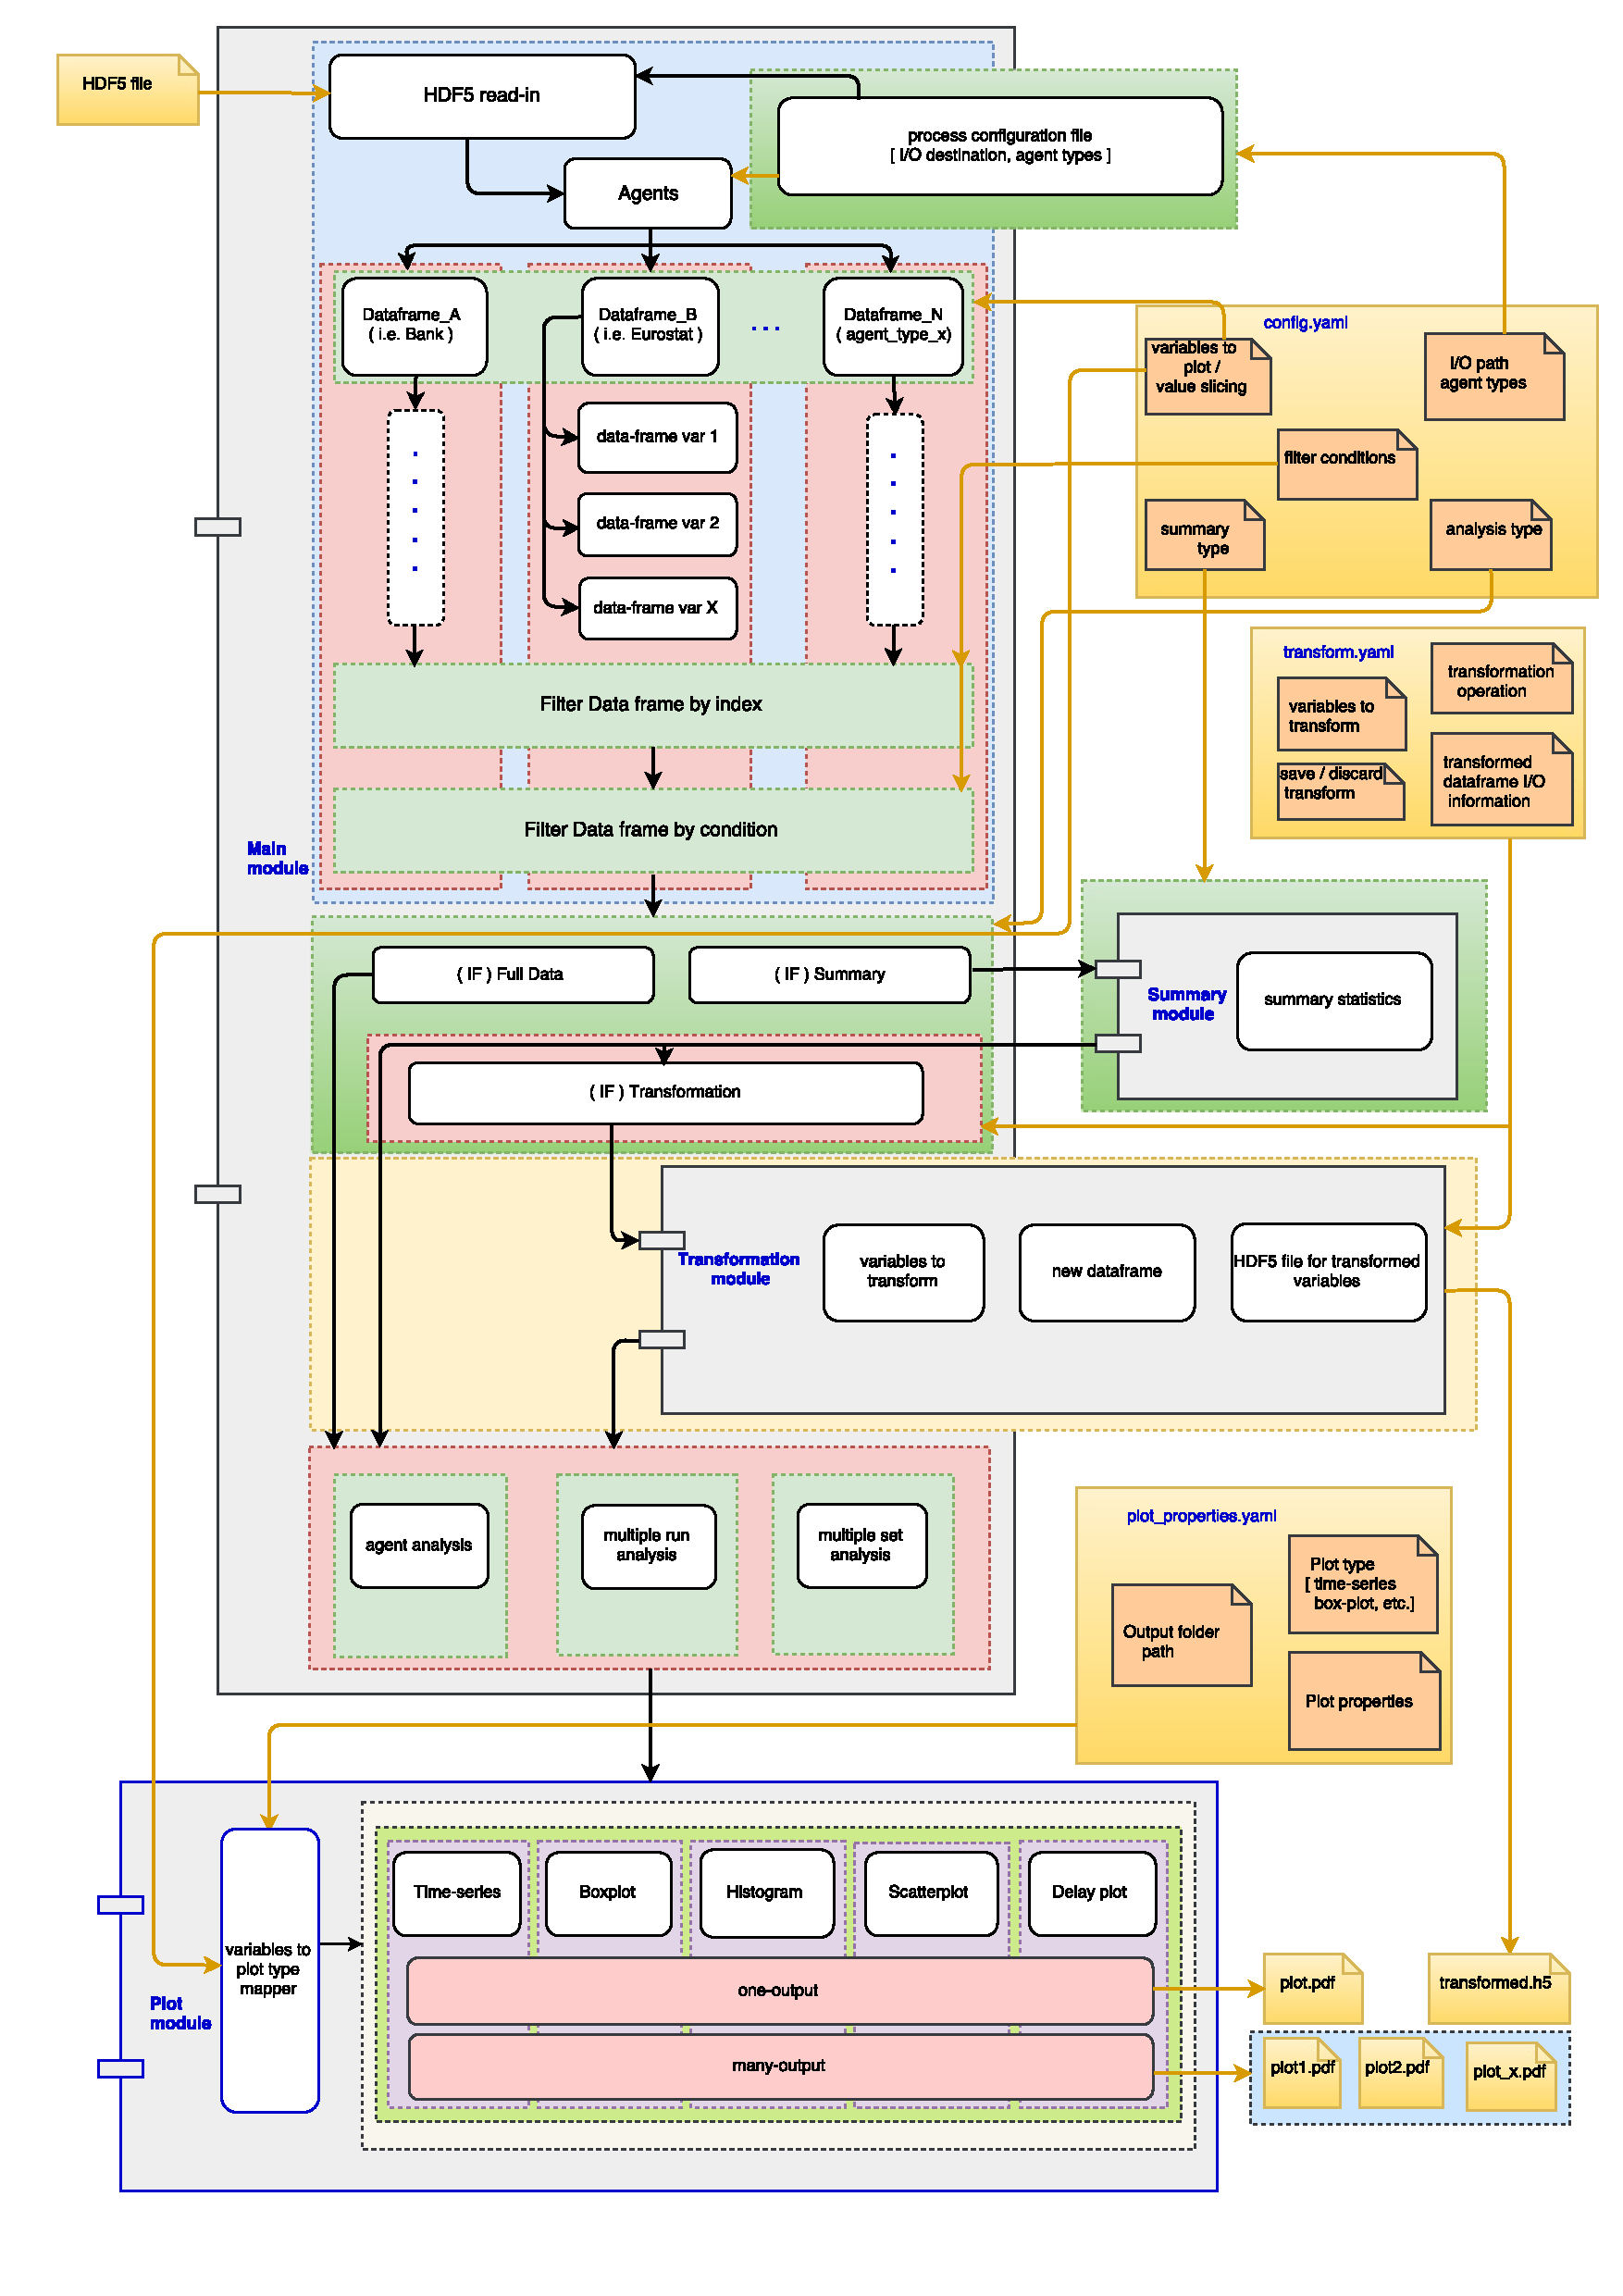
\includegraphics[scale=0.40]{flame_pandas_workflow_diagram.pdf}
\end{minipage}
\end{figure}
\end{frame}
\note{
\textbf{Flame with pandas workflow diagram (cont.)}

\underline{Module Yellow:} Data transformation module

g. Data transformations: simple arithmetic operations (+,-,*,/) on any available data

h. Output a new data frame (in RAM) with for newly created variables (ratios, growth rates, sums, statistics, ...)

i. Output a new HDF5 file to disk after data transformations are done

\underline{Module Red:} Data preparation module

j. Data preparation: depending on the type of analysis (agent-level, run-level, ensemble-of-runs, set-level, ensemble-of-sets)

\underline{Module Green:} Plotting module

k. Data visualization: produce plots depending on the type of visualization (views) and whether you want a single file (multiple lines per plot) or multiple files (single line per plot)
}

%--------------------------------------------------------------------------
\section{Data visualization}
%--------------------------------------------------------------------------

\begin{frame}{}\small
\frametitle{Time series plot: multiple agents, 1 variable, 1 set, 1 run\\(2D - time series of 20 agents)}

\begin{figure}[hb!]
\centering\leavevmode
\graphicspath{{./png/plots/time_series/agent_level/}}
%
\hspace{-4cm}
\begin{minipage}{10cm}
\centering\leavevmode
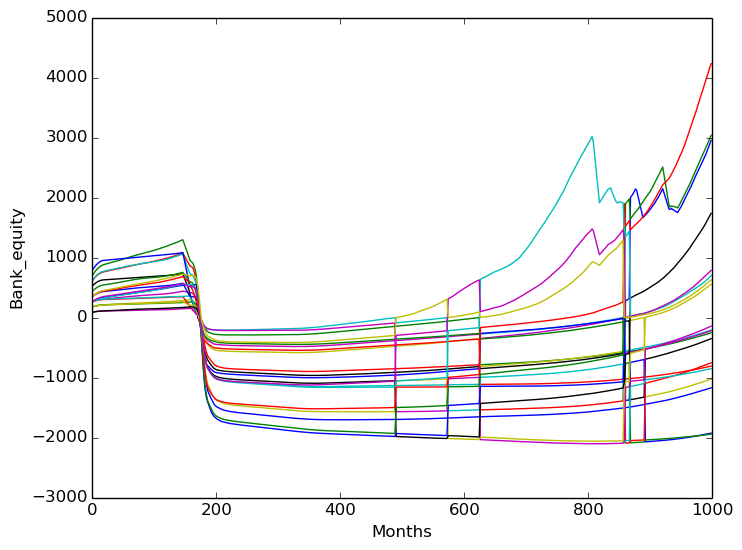
\includegraphics[scale=0.45]{[Set2]_Bank_1_set_1_run_20_instance.png}
\end{minipage}
\end{figure}
\end{frame}
\note{
This plot shows:

- the data for this plot is 2D

- the data is for 20 agents, 1 variable, 1 set, 1 run

- we plot the time series for each agent individually.
}

%--------------------------------------------------------------------------

\begin{frame}{}\small
\frametitle{Time series plot: multiple agents, 1 variable, 1 set\\(3D - quantiles across agents + 20 runs)}

\begin{figure}[hb!]
\centering\leavevmode
\graphicspath{{./png/plots/time_series/Bank_plots/set_2/}}
%
\hspace{-4cm}
\begin{minipage}{10cm}
\centering\leavevmode
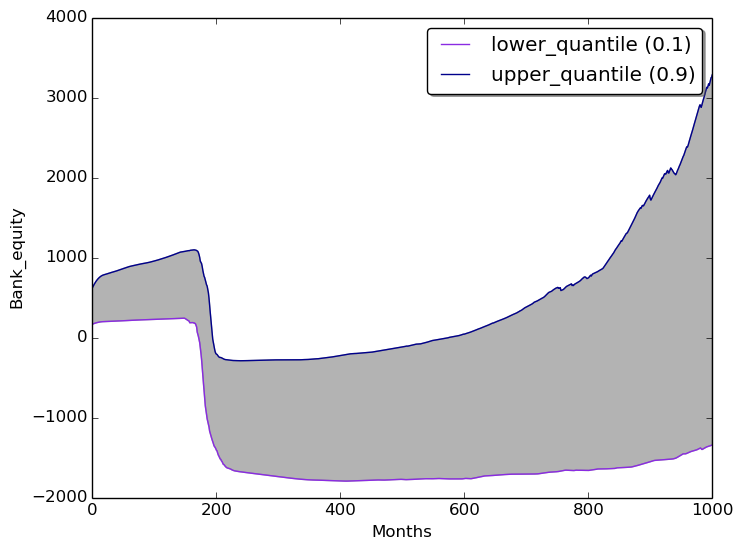
\includegraphics[scale=0.45]{Bank_equity_1_set_20_run(set2_unstable_case).png}
\end{minipage}
\end{figure}
\end{frame}
\note{
This plot shows:

- the data for this plot is 3D

- the data is for 20 agents, 1 variable, first gets collected in an ensemble distribution: all observations at one point in time are combined

- this is done for 20 runs, so in principle the underlying data consists of 400 time series (20 runs, 20 agents).

- and then we take the quantiles across these 400 data sets
}

%--------------------------------------------------------------------------

\begin{frame}{}\small
\frametitle{Time series plot: multiple agents, 1 variable, 2 sets\\(4D - quantiles across 20 runs)}

\begin{figure}[hb!]
\centering\leavevmode
\graphicspath{{./png/plots/time_series/Bank_plots/set_1/}}
%
\hspace{-4cm}
\begin{minipage}{10cm}
\centering\leavevmode
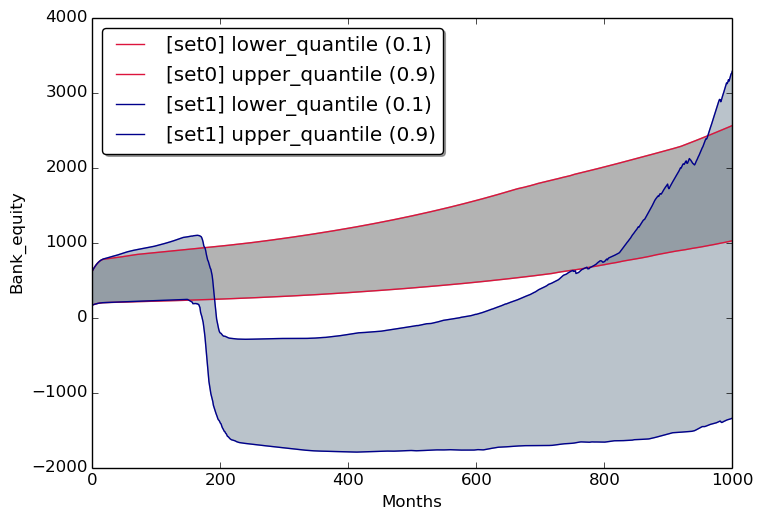
\includegraphics[scale=0.45]{Bank_equity_2_set_20_runs_quantile.png}
\end{minipage}
\end{figure}
\end{frame}
\note{
This plot shows:

- the data for this plot is 4D

- the same type of plot as in the previous slide, but now for 2 parameter sets.
}

%--------------------------------------------------------------------------

\begin{frame}{}\small
\frametitle{Time series plot: multiple types, multiple agents, 2 variables, multiple runs, 1 set (5D - time series of ensemble quantiles)}

\begin{figure}[hb!]
\centering\leavevmode
\graphicspath{{./png/plots/time_series/Bank_Firm_joint_plots/}}
%
\hspace{-4cm}
\begin{minipage}{10cm}
\centering\leavevmode
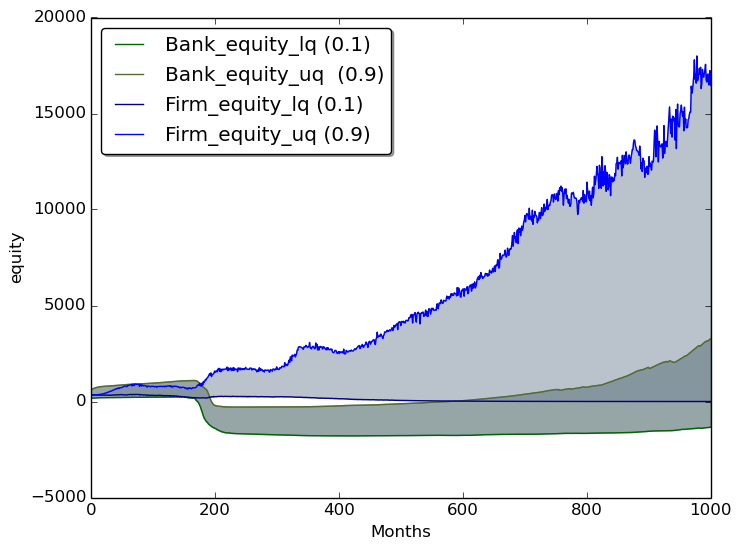
\includegraphics[scale=0.45]{[set_2]_Bank_Firm_equity_1_set_20_runs_quantile.png}
\end{minipage}
\end{figure}
\end{frame}
\note{
This plot shows ensemble quantiles over time:

- the data for this plot is 5D

- here we have multiple agent types: Bank and Firm

- each type has multiple agents, so we collect their time series over 20 runs

- then we consider the ensemble: 20 banks + 80 firms -> 2,000 data series in total

- and plot the quantiles of Bank.equity (400 series) and Firm.equity (1600 series), at each point in time

- the data for this plot is the same as for the boxplot, but we plot the entire time series evolution of the agent distribution of the variable, and we do this for two different agent types, and two different variables.
}

%--------------------------------------------------------------------------

\begin{frame}{}\small
\frametitle{Box plot: multiple agents, 1 variable, multiple runs, 1 set\\(3D - box plots of ensemble distribution across agents + 20 runs)}

\begin{figure}[hb!]
\centering\leavevmode
\graphicspath{{./png/plots/time_series/Bank_plots/set_1/}}
%
\hspace{-4cm}
\begin{minipage}{10cm}
\centering\leavevmode
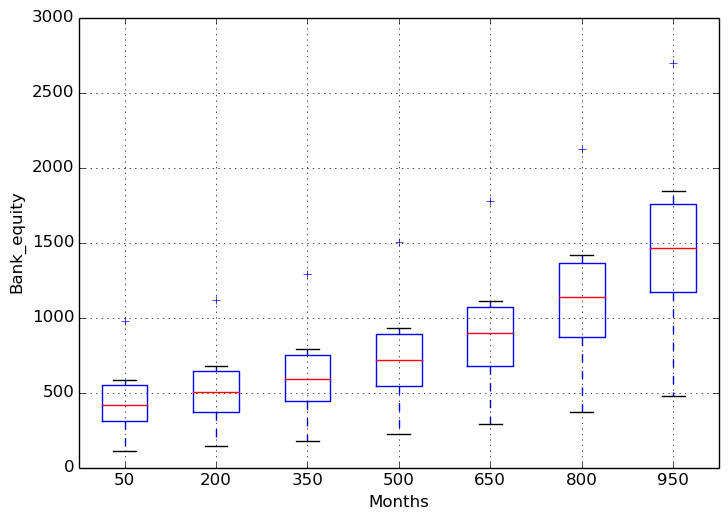
\includegraphics[scale=0.45]{Bank_equity_1_set_20_runs_boxplot.png}
\end{minipage}
\end{figure}
\end{frame}
\note{
This plot shows box plots of an ensemble distribution of data:

- the data for this plot is 3D

- for multiple agents, we collect their data series across 20 runs

- then we consider the ensemble: 400 data series in total

- and we plot a box plot at selected points in time

- each box plot shows the ensemble across all agents and across all 20 runs
}

%--------------------------------------------------------------------------

\begin{frame}{}\small
\frametitle{Some Performance Metrics (Memory consumption, 100 sets) }

\begin{figure}[hb!]
\centering\leavevmode
\graphicspath{{./png/Benchmarks/}}
%
\hspace{-4cm}
\begin{minipage}{10cm}
\centering\leavevmode
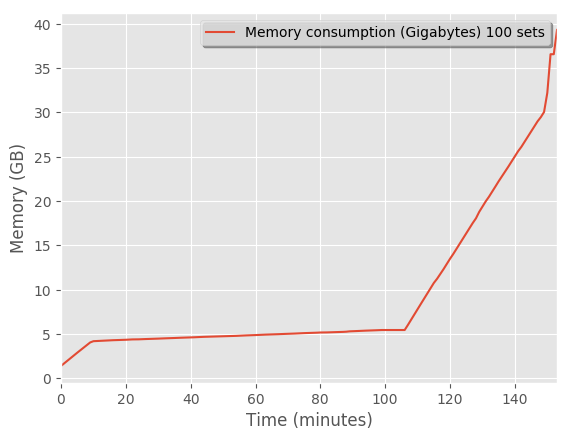
\includegraphics[scale=0.55]{Fig_100.png}
\end{minipage}
\end{figure}
\end{frame}


%--------------------------------------------------------------------------

\begin{frame}{}\small
\frametitle{Some Performance Metrics (Memory consumption, 250 sets) }

\begin{figure}[hb!]
\centering\leavevmode
\graphicspath{{./png/Benchmarks/}}
%
\hspace{-4cm}
\begin{minipage}{10cm}
\centering\leavevmode
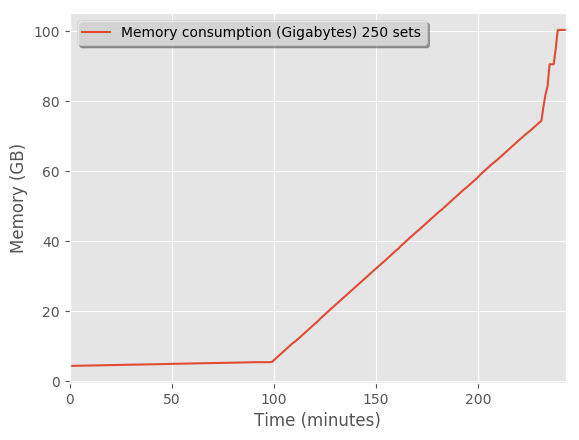
\includegraphics[scale=0.55]{Fig_250.png}
\end{minipage}
\end{figure}
\end{frame}


%--------------------------------------------------------------------------

\begin{frame}{}\small
\frametitle{Some Performance Metrics (Memory consumption, 513 sets) }

\begin{figure}[hb!]
\centering\leavevmode
\graphicspath{{./png/Benchmarks/}}
%
\hspace{-4cm}
\begin{minipage}{10cm}
\centering\leavevmode
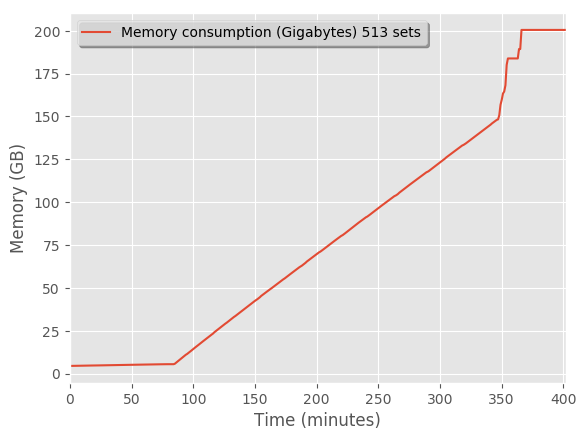
\includegraphics[scale=0.55]{Fig_513.png}
\end{minipage}
\end{figure}
\end{frame}


%--------------------------------------------------------------------------

\begin{frame}{}\small
\frametitle{Some Performance Metrics (Memory consumption, comparing three cases) }

\begin{figure}[hb!]
\centering\leavevmode
\graphicspath{{./png/Benchmarks/}}
%
\hspace{-4cm}
\begin{minipage}{10cm}
\centering\leavevmode
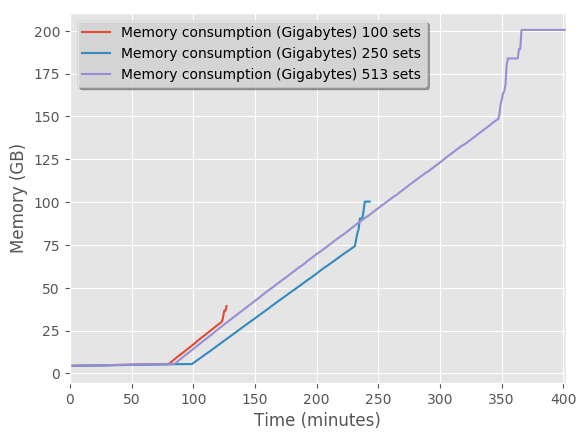
\includegraphics[scale=0.55]{Fig_all.png}
\end{minipage}
\end{figure}
\end{frame}


%--------------------------------------------------------------------------

\section{Summary}
%--------------------------------------------------------------------------
\begin{frame}{}\small
\frametitle{Summary}

\begin{enumerate}\itemsep2em

\item Software library for ABM Data Analysis using Python pandas

\item General-purpose tool for analysing ABM data

\end{enumerate}
\vspace{0.7cm}
\textbf{Re-stating the important question: How to fit it all together (given the context of CONQUAIRE)!}
\newline

\begin{enumerate}\itemsep2em

\item How is it to be integrated in the Conquaire workflow; also what measures of Quality Control for our particular case?

\item What are the requirements (expected of us) for the proposed Quality Control?


\end{enumerate}
\end{frame}
\note{no notes
}

%--------------------------------------------------------------------------

\section{EndPage}
%--------------------------------------------------------------------------
\begin{frame}{}\small
\vspace{1cm}
\begin{center}
\huge{Suggestions / Discussion / Questions ?}
\end{center}
\end{frame}
\note{no notes
}


%--------------------------------------------------------------------------
% Appendix: Reserve slides
%--------------------------------------------------------------------------

\begin{frame}{}\small
\frametitle{Data Volume Table}

\begin{figure}[hb!]
\centering\leavevmode
\graphicspath{{./png/}}
%
%\hspace{-4cm}
\begin{minipage}{10cm}
\centering\leavevmode
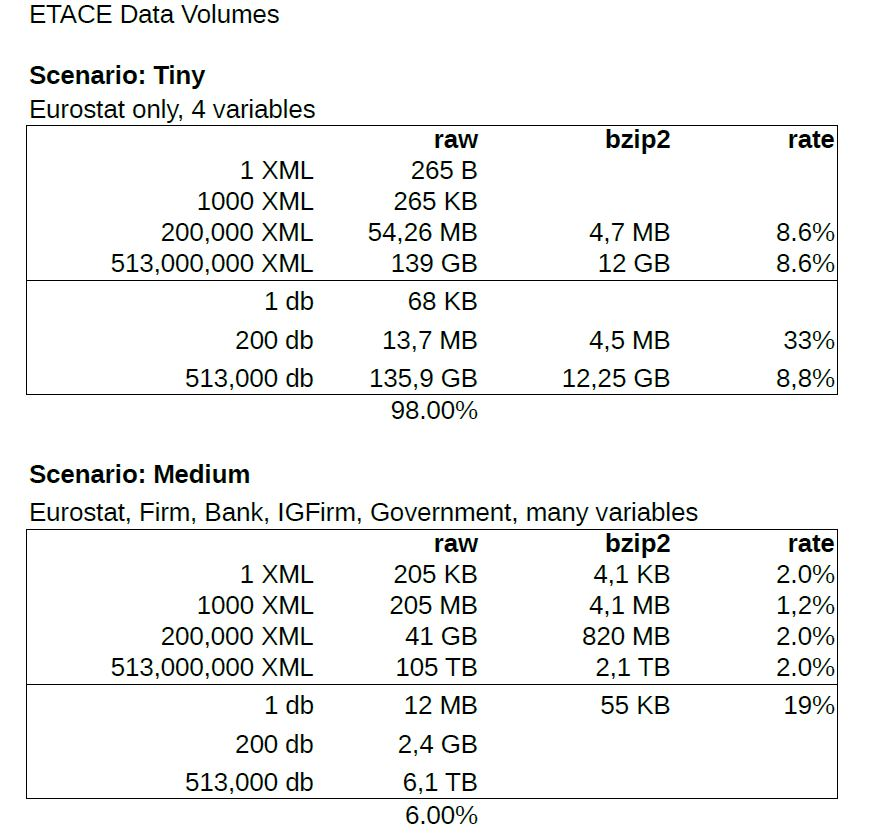
\includegraphics[scale=0.4]{table_data_volumes.jpg}
\end{minipage}
\end{figure}
\end{frame}
\note{}


\end{document}

%--------------------------------------------------------------------------
% Appendix: Template slides
%--------------------------------------------------------------------------
\begin{frame}{}\small
\frametitle{}

\begin{enumerate}\itemsep2em

\item 

\item 

\item 
 
\end{enumerate}
\end{frame}
\note{
}

%--------------------------------------------------------------------------

\begin{comment}
\begin{frame}{}\small
\vspace{-1cm}
\thispagestyle{empty}
\textbf{Title}

\begin{figure}[hb!]
\centering\leavevmode
\graphicspath{{../png/}}
%
\begin{minipage}{16.5cm}
\hspace{-1cm}
%
\begin{minipage}{3cm}
\centering\leavevmode
%{\small $t=0$}
%\includegraphics[width=3cm]{cuttlefish_0000.pdf}
\end{minipage}
%
\end{minipage}
\caption{}
\end{figure}
\end{frame}
\end{comment}


\end{document}